% experiments.tex

\iffalse
\cs{under construction}
\begin{itemize}
	\item Object detection models in CV have different goal than L+V object recognition models (see related work--former is on labels, latter on predicting natural language). 
	However, the former, pre-trained towards labels, are the backbone / used as feature extractors for the latter.
	\item ... 
	\item As we explained, there is a high variation of object names, and objects may be named by multiple alternative names (\cs{vocab size MN vs. vocab size VG for same object set}). 
	Yet, humans usually have a clearly preferred name for individual object instances (and the set of those is relatively small)--humans agree on a particular name for an instance (entry-level name).
	\item Hence, to model human object naming, datasets with many/dozens of annotations for the same instance are required. 
	\item We argue that such datasets are more reliable in that they provide empirically derived preferred names (entry-level names), and richer--the provide valid name alternatives. 
	\item But since their elicitation is expensive and time-consuming, it is not realistic to create training datasets of dozens of object names for pre-training features with CV models, which need a huge amount of training data. 
\end{itemize}
\fi

We propose to use datasets of object names for evaluating models on the task of object naming (depending on results: also valuable for comparing object detection/image classification models).
Specifically, we analyse object detection [and classification] models on the task of human object naming, using the \mn dataset as test data:\\
Can object detection models, trained on arbitrary names, account for human object naming?
\begin{itemize}
	\item Do they predict the entry-level name?
	\item Are valid name alternatives among the top-N predictions?
	\item Do models make similar mistakes as humans when being faced with the task of naming highlighted objects in images [i.e.,\ the artificial setup of object naming for data annotation]?\\
	-- naming an alternative object (maybe more salient)\\
	-- predicting a semantically related name
	%do we get different evaluation results when testing existing object classification models on preferred responses from name distributions, as compared to naming responses collected from 1-3 workers (e.g., VisualGenome)? 
	\item Can we use \mn as fine-tuning dataset? (Here: only Vanilla model)\\
	-- can we learn entry-level names by fine-tuning object detection models on \mn?\\
	-- Can we directly learn entry-level names by fine-tuning image classification models on \mn, i.e.,\ the pre-trained features to initialize object detection models?
\end{itemize}

\subsection{Experimental Setup}
\label{sect:exp_setup}

\paragraph{Data}

\paragraph{Models}

\paragraph{Measures}


\subsection{[TBC] Predicting Entry-Level Names}
\label{sect:exp_entry}
Question: Can object detection models trained on a set of "arbitrarily" chosen object names account for entry-level object names? 

Note that the source dataset for defining the vocabulary (\textsl{Vocab}, i.e.,\ the overall set of considered names, i.e., the softmax layer's dimensions), and the source dataset which provides the ground truth names for the individual objects (\textsl{GTtrain}) may differ.  

\begin{table*}[t]
	\centering
	\small
	\begin{tabular}{l|c|r@{~}r@{~}r@{~}r@{~}r@{~}r@{~}r|@{~}r@{~}r@{~}r@{~}r@{~}r@{~}r@{~}r@{~}}
		\toprule
		&   & \multicolumn{6}{c}{All Test Images ($\#$)} 
		& \multicolumn{6}{c}{VG$\neq$MN Images ($\#$)}\\	
		Model--Vocab	 
		&  GTtrain &  =VG & =MN & $\in$MN  & KL & J & MRR & AvgMRR 
		&  =VG & =MN & $\in$MN  & KL & J & MRR & AvgMRR\\ 
		\midrule
		FRCNN--VG2500 & VG \\
		FRCNN--VG1600 & VG & \\
		FRCNN--MN442 & VG &   \\
		\midrule \midrule
		& \multicolumn{12}{c}{Classifiers: Fine-tuning pre-trained image features on \mn}\\
		Features--Vocab & GTtrain  \\
		\midrule 
		FRCNN--VG1600--VGMN & MN &  \\
		& MN-12ep  &           \\ 
		FRCNN--VG1600--MN442 &  MN \\
		\midrule
		ResNet101--VGMN\_4ep  &   VG  \\
		ResNet101--VGMN\_8ep & VG &  \\
		ResNet101--VGMN & MN \\
		ResNet101--MN442 & VG \\
		ResNet101--MN442 & MN &\\
		\bottomrule
	\end{tabular}
	\caption{Target vocabulary in test data: MN442. Vocab denotes the dataset from which the target vocabulary for training was induced (the numbers give the size of the vocabulary). GTtrain denotes the dataset from which the ground truth labels are obtained during \textit{training}. MRR is mean reciprocal rank; J is Jaccard score.\label{tab:entrylevels}. }
\end{table*}


\subsection{[TBC] Humans vs. Models: Which Mistakes do they Make?}
\label{sect:exp_analysis}

\paragraph{Categorization of Errors}
see Figure\ ref{fig:mistakes}
\begin{enumerate}
	\item Clear mistake \\
	e.g.,\ rice vs. bread
	\item Alternative name\\
	e.g.,\ building vs. house
	\item Alternative object \cs{(other cluster from verif data)}
	\item Synonym\\
	e.g.,\ plane vs. airplane
	\item Semantically related\\
	e.g.,\  motorcycle vs. scooter
\end{enumerate}

\begin{figure}
	\centering
	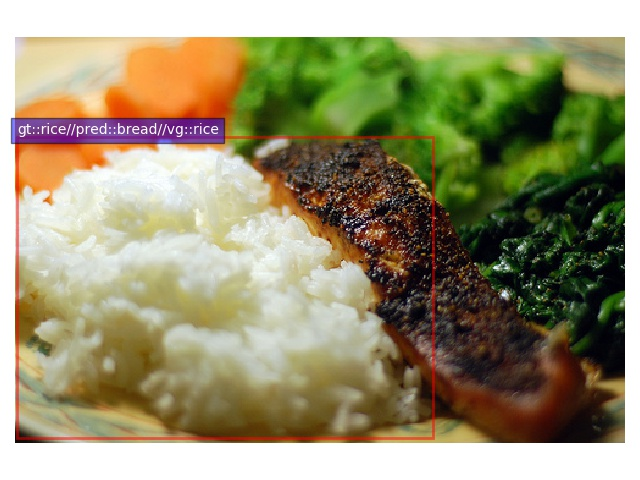
\includegraphics[scale=.2]{images/2323938.jpg}
	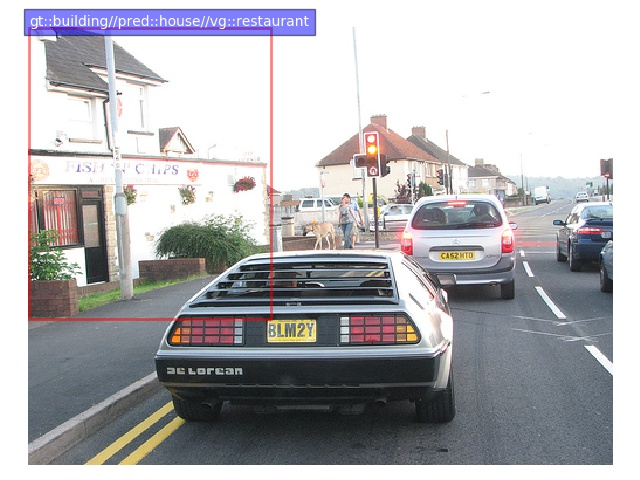
\includegraphics[scale=.2]{images/2322259.jpg}
	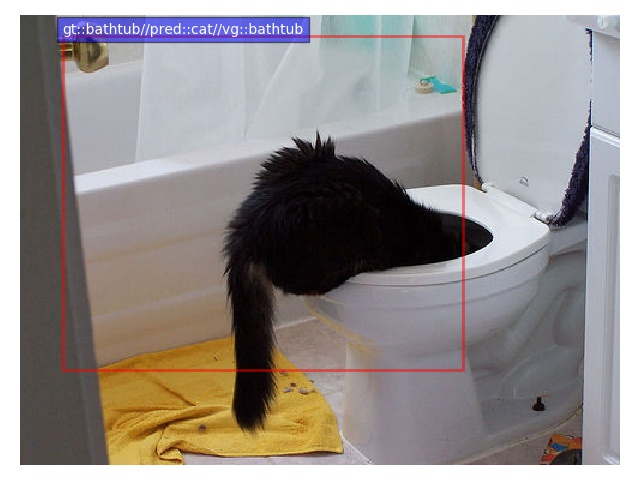
\includegraphics[scale=.2]{images/2371657.jpg}
	
	\caption{resnet mistakes (trained on vg\_manynames, tested on manynames-442)\label{fig:mistakes}}
\end{figure}


\subsection{[TBC] Generalization Ability: OpenImages}
\label{sect:exp_openimages}
Question: Can models trained towards \mn generalize to other, related datasets? Here: OpenImages. \cs{[Increase coverage with zero-shot learning?]}\

Models compared: FRCNN--VG1600 vs. FRCNN--MN442 vs. ResNet101--XX (best Vanilla).
